\documentclass[12pt]{article}
\usepackage{listings}
\usepackage[pdftex]{graphicx}


\pagestyle{empty}
\setcounter{secnumdepth}{2}

\topmargin=0cm
\oddsidemargin=0cm
\textheight=22.0cm
\textwidth=16cm
\parindent=0cm
\parskip=0.15cm
\topskip=0truecm
\raggedbottom
\abovedisplayskip=3mm
\belowdisplayskip=3mm
\abovedisplayshortskip=0mm
\belowdisplayshortskip=2mm
\newcommand{\tab}{\hspace*{2em}}
\normalbaselineskip=12pt
\normalbaselines

\begin{document}

\vspace*{0.5in}
\centerline{\bf\Large Test Document}

\vspace*{0.5in}
\centerline{\bf\Large Team 1}

\vspace*{0.5in}
\centerline{\bf\Large 8 April 2012}

\vspace*{1.5in}
\begin{table}[htbp]
\caption{Team}
\begin{center}
\begin{tabular}{|r | c|}
\hline
Name & ID Number \\
\hline\hline
Jonathon Bergeron & 9764453 \\
Marc-Andre Faucher & 9614729 \\
Jeffrey How & 9430954 \\
Dmitry Kuznetsov & 5679311 \\
Willian Ling & 9193480 \\
Thomas Paulin & 9333630 \\
Alain Sakha & 9770836 \\
Kai Wang & 5652723 \\
\hline
\end{tabular}
\end{center}
\end{table}

\clearpage

\section{Introduction}

{
This testing plan document outlines the testing to be done on the system that ensures that it meets specified requirements in a proper, organized way, and provides a reasonable user experience within those requirements and that feature set. \\

Specifically, the goals of this document are to formulate a scheduled plan to thoroughly validate that system requirements are met at the system, subsystem and unit levels, along with the inclusion of integration and regression testing, and to list the results of these tests in a manner in which the requirements they meet are known. Additionally, this document aims to verify that the way in which the requirements are implemented provides a certain feature set that has the ability to surprise and delight users. \\

The information contained in this document includes a brief overview of the forms of testing done on the system, the schedule and resources required and used for testing, brief notes on the design of the test cases, as well as detailed test results at each aforementioned level, along with their results and the system requirements which they are intended to satisfy. \\
}



\section{Test Plan}

{
The testing planned for the system spans the various levels of production. As the system was tested starting at the unit level, the method of testing was bottom up. Regardless, the tests will be outlined in a top-down fashion, based on the complete design and integration of the system. \\
}

\subsection{System Level Test Cases}
{
These system test cases define overarching test cases for the software that are designed to test both the design and behavior of the system and its main functional requirements. Specifically, detailed scenarios will be covered in the sections describing subsystem and unit tests.
}
\subsubsection{Test Case 1 - System Execution}
\begin{quote}
{\bf Purpose}
{
The purpose of this system test is to ensure the user can run the program on all platforms capable of running the Java Virtual Machine (JVM).
}
\\
{\bf Input Specification}
\\
{
For this case, there is no input files or methods needed to be called. The test simply is designed to ensure that the application is portable, and thus can execute on any system configuration capable of running the JVM.
}
\\
{\bf Expected Output}
\\
{
The system is expected to be able to run the application regardless of hardware and software configuration, including, but not limited to Windows (XP/Vista/7, 32 bit and 64 bit), Max OS X (10.X), various Linux distributions, etc.
}
\\
{\bf Traces to Use Cases}
\\
{
This system test relates directly to the non-functional requirement O1 from the requirements document (also included in Appendix C) which states ``It shall be possible to run the system on any computer system that run the JVM."
}
\end{quote}

\subsubsection {Test Case 2 - System Navigation and Use}
\begin{quote}
{\bf Purpose}
\\
{
The purpose of this system test is to ensure the user has access to all system functions, interface options, and generally can perform any given specified requirement of the system. \\
}
{\bf Input Specification}
\\
{
For this case, there are no explicit input files that need to be inputted to the system. All system XML files, however, need to be included as expected with the system. The files, people.xml and task.xml, can be found in detail in the Appendix A at the end of this document
}
\\
{\bf Expected Output}
\\
{
The system is expected to be able to run without error, and the user has access to all tabs (Tasks, People, Gantt Chart, and Tree View) and can perform all operations on each tab. These cases will be explained in greater detail in the subsystem and unit level test descriptions, and the only scenario in which an output file is produced can be found in Appendix B (people.txt).
}
\\
{\bf Traces to Use Cases}
\\
{
The system test should validate all use cases, scenarios and requirements implemented for the system. Specifically, the requirements F2 - F13 as specified by the requirements document, and included for reference in Appendix C.
}
\end{quote}

\subsection{Subsystem Level Test Cases}
{
The subsystem tests for the system are designed to test specific collections of units of functionality within the system. As the system separates requirements by the Model, View, Controller architecture, those will serve as the major subsystems of the system.
}
\subsubsection{Model Subsystem}
\begin{quote}
{\bf Purpose}
\\
{
The purpose of this system test is to ensure the data model always maintains integrity and is not affected by the operations performed by user. While data will change, the way the data it stored should not be affected.
}
\\ 
{\bf Input Specification}
\\
{
For this test case, the input specification should simply be valid format XML files. As long as the system is able to process the files, the data should be stored properly in appropriate data structures.
}
\\
{\bf Expected Output}
\\
{
The system is expected to function using the proper data format in combination with their storage in proper data structures.
}
\\
{\bf Traces to Use Cases}
\\
{
This test case does not directly relate to any functional or non-functional requirements, however is implicitly essential to all requirements and functionality.
}
\end{quote}
\subsubsection{View Subsystem}
\begin{quote}
{\bf Purpose}
\\
{
The view subsystem is designed to handle all the required display options for the data. This includes the tree view, gantt chart, tables, etc.
}
\\
{\bf Input Specification}
\\
{
For this test case, the input specification should simply be valid format XML files. As long as the system is able to process the files, the view should be able to accurately display regardless of which option is selected, and how the data is changed in the model.
}
\\
{\bf Expected Output}
\\
{
The system is expected to function by displaying any requested view to the user using the data specified in the model.
}
\\
{\bf Traces to Use Cases}
\\
{
The view subsystem has several direct traces to use cases and requirements of the system. Specifically, functional requirements F2, 6, 7, 10 as indicated in Appendix C and the requirements document. These functional requirements dictate the many ways in which the data can be displayed graphically to the end user.
}
\end{quote}

\subsubsection{Controller Subsystem}

\begin{quote}
{\bf Purpose}
\\
{
The controller subsystem is designed to perform operations on the model as dictated by the operations the user performs on the view. This includes update XML files, output text files, etc.
}
\\
{\bf Input Specification}
\\
{
The input XML files should simply be of valid format. Any data combinations should work. The workflow process can begin at one of many points, including the addition/removal of tasks or employees, modification of employees, etc.
}
\\
{\bf Expected Output}
\\
{
The system is expected to function by appropriately modifying data stored in structures, and any needed XML files. Specific units need to be tested as the process continues.
}
\\
{\bf Traces to Use Cases}
\\
{
As evidenced by its purpose and input/output specifications, the controller subsystem is related directly to several functional requirements. These requirements are as follows: F3, F4, F5, F8, F9, F11, F12, F13, all described in Appendix C.
}
\\
\end{quote}

\subsection{Unit Test cases}
{
The unit and their tests desrcibed in this section represent the individual methods of the system, most of which are small and inputs predictable. Details follow.
}


{\bf updateXML()}
{
Test for if people or task are empty; 
}

{\bf getTaskData()} 
{
Test if a task object is empty or null
}

{\bf getPeopleData()} 
{
Test if a person object is empty or null
}

{\bf getTotalHoursOnProjects()} 
{
Test if the total hours on a project is negative, or if the testing total hour is same as expected value.
}

{\bf getListOfProjects()}
{
Test if the project list is empty or null, and check if the output vaue is the same as expected value.
}

{\bf nextAvailableId()}
{
Test if the nextAvailableID() is proper value or null
}

{\bf findTask()}
{
Test if by using the taskID, we can get the expected task
}

{\bf assignStringOfID()} 
{
Test if the assigned ID is the expected ID.
}

{\bf testSetIdentifier()}
{
Test if the identifier fits its proper type pattern.
}

{\bf testSetFName()}
{
Test if the first name fits its proper type pattern.
}

{\bf testSetLName()}
{
Test if the last name fits its proper type pattern. 
}

{\bf testSetJobTitle()}{
Test if the job title fits the proper type pattern.
}

{\bf testSetJobDescription()}{
Test if the job description fits the proper type pattern.
}

{\bf testSetTotalHours()}{
Test if the total hours set for a project is an integer number.
}

{\bf testSetCompletion()}{
Test if completion is a percentage number.
}

{\bf testSetDeadline()}{
Test if the deadline is a valid date.
}

{\bf testSetParent()}{
Test if the parent ID is a valid ID.
}

{\bf testSetParentDependencyID()}{
Test if the parent dependency ID is a valid ID. 
}

{\bf testSetStartDate()}{
Test if the start date is a valid date.
}

{\bf testSetDeliverable()}{
Test if the deliverable follows correct type pattern.
}

{\bf testSetDescription()}{
Test if the description follows correct type pattern.
}

{\bf testSetDuration()}{
Test if duration is an integer number.
}

{\bf testSetIdentifier()}{
Test if the Identifier ID is an integer number.
}

{\bf testSetPeopleAssignedarray()}{
Test if all the ID's of people assigned are integers.
}

{\bf testSetTitle()}{
Ensure that the title being set is valid according to its type.
}

\begin{figure}[htbp]

\begin{center} 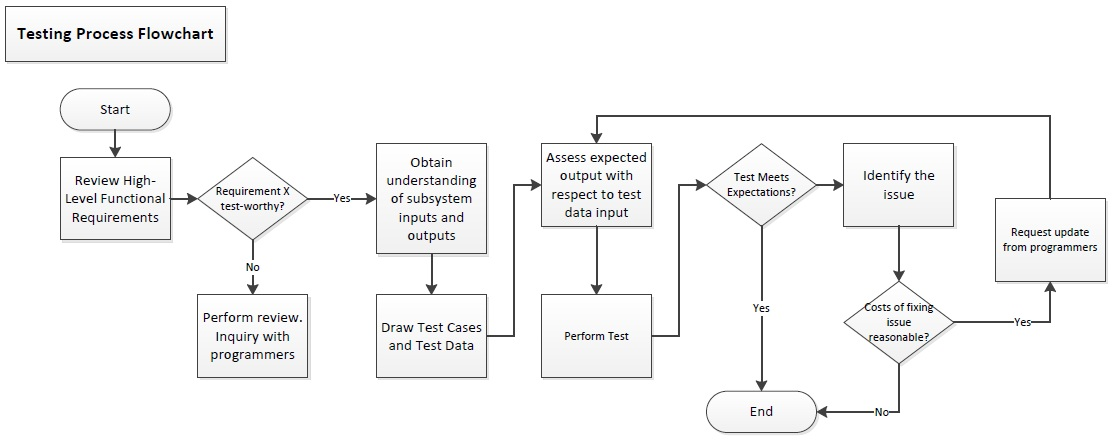
\includegraphics[scale=.6]{TestDiagram.jpg} \end{center}
\label{fig:testing-diagram}
\caption{Sample Flow for unit testing}

\end{figure}

\subsection{Regression Testing}
{
Regression testing performed on the system involved ensuring that all previous code and functionality is not affected after changes made for the current increment. The regression tests were divided into three major test cases, file format validation, MVC architecture validation, and functionality verification.
}
\subsubsection{Test Case 1 - XML File Formats Validation}
\begin{quote}
{\bf Purpose}
\\
{
The purpose of this regression test is to ensure that the validation methods on the XML data format still function as intended and can handle erroneous cases.
}
\\
{\bf Input Specification}
\\
{
The system state should be normal, reading in the XML files as intended. The regression test includes invalid file formats specified through unit tests. These invalid XML files are attached and part of the Appendix A.
}
\\
{\bf Expected Output}
\\
{
The expected system response is to be able to handle and report appropriate data errors. For most cases, blank fields, unclosed tags on non-critical fields will be handled by the system in a manner that allows the user to continue on execution and operation of all intended functionality. For certain critical fields, such as user ID, task ID, hours assigned, etc. invalid XML formats will be handled in a way by the system that removes that record from operation, and allows the user to continue operation and execution of the system with other, valid records. In both cases the only system output is console-level error messages, detailing how the system recovered from the error.
}
\\
{\bf Traces to Use Cases}
\\
{
This test case does not satisfy an explicit user requirement or use case, but does satisfy an implicit system requirement, that the XML input files must be readable, and the system must be able to survive data errors in a user-friendly way.
}
\end{quote}
\subsubsection {Test Case 2 - MVC Architecture Validation}
\begin{quote}
{\bf Purpose}
\\
{
The purpose of this regression test is to ensure that the Model View Controller architecture implemented in Increment 2 is not affected by the changes made in implementing Increment 3 functionalities
}
\\
{\bf Input Specification}
\\
{
The system state should be maintained in a way that separates the data from the user interface and the methods that manipulate it. There is no specific input file needed, other than the default, valid XML file needed for normal program execution.
}
\\
{\bf Expected Output}
\\
{
The system is expected to function as normal. There is no specific output other than the user being able to view each view properly as they manipulate data. The pople.txt output file should be produced as normal.
}
\\
{\bf Traces to Use Cases}
\\
{
This test case does not satisfy an explicit user requirement or use case, but does satisfies an implicit requirement that the MVC architecture is used to implement the system.
}
\end{quote}
\subsubsection{Test Case 3 - Functionality Verification}
\begin{quote}
{\bf Purpose}
\\
{
The purpose of this regression test is to ensure that all previous functionality available in previous increments is still available and working correctly with the changes added by the current increment.
}
\\
{\bf Input Specification}
\\
{
The system state should be viewed as normal, that is, a regular execution is expected with all exceptions handled. The default input should be used, which includes generic, valid input XML files.
}
\\
{\bf Expected Output}
\\
{
The expected system response is to be able to perform the functionalities added in Increments 1 or 2, including being able to produce a valid people.txt file, and the view of the people, and tasks table, and any operations able to be
}
\\
{\bf Traces to Use Cases}
\\
{
This requirement has several traces to use cases and requirements, specifically requirements: F2, F3, F4, F5, F8, F10. Detailed information for requirements are available in Appendix C.
}
\end{quote}
\subsection{Integration Testing}
{
Implementation testing was performed as components were added to the system. While there are no specific test cases, the regression test were run as components were added.

As stated earlier, the system was implemented in a bottom-up manner, meaning that modules were slowly coupled together, and implemented beginning at the unit. Below is a diagram of the way in which the modules of the system were integrated:

\begin{figure}[htbp]

\begin{center} 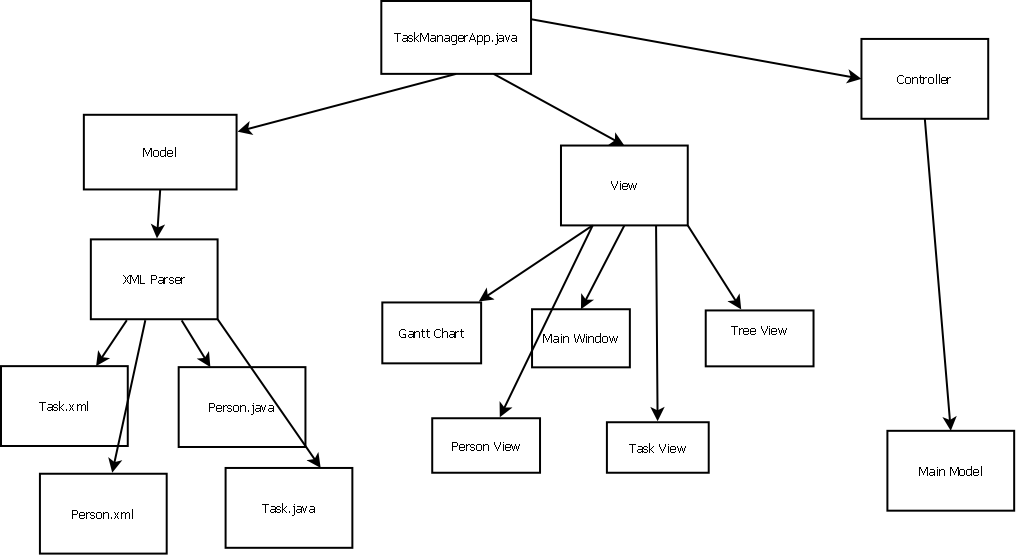
\includegraphics[scale=.3]{inc3_bottomup.png} \end{center}
\label{fig:bottom-up-diagram}
\caption{Bottom-Up Integration of System}

\end{figure}

}
\subsection{Schedule and Resources for Testing}
{
This section defines the schedule and resources used in the testing of the system.
}

\subsection{Notes on Test Case Design}
{
The test cases were designed to be operated within the confines of the MVC system, meaning that each case was written and performed keeping the notion of a separate Model, View and Controller in mind. This means that test cases need to ensure that each separate portion of the system maintained integrity both as a whole, and separately.
}

\subsection{Requirements Tested and Omitted}
\subsubsection{Requirements Tested} \label{rt:1}
       
{
The requirements tested in the development of the system are listed in the requirements document and in Appendix C of this document. The specific requirements are labeled functional requirements F2-F10, F13, as well as operational requirement O1, with the omission of functional requirement F1, F11, F12 covered in detail below.
}

\subsubsection{Requirements Omitted} \label{rt:2}

{
The requirements listed in the requirements document (included in Appendix C) omitted from the testing and eventual development of the system are requirements F1 and N1.

Functional requirement F1 states ``Only one person should be logged in at a time." This requirement was later dropped from development during the development of Phase 2, as it was deemed beyond the scope of the application, as the application functioned better in a more general form. This functionality was thus not tested as part of the requirements.

Functional requirement F11, F12 were discarded, as the notion of administrator users was omitted as part of F1. As this is the case,

Non-functional requirement N1, specifically ``the system must know who the user is in order to order the appropriate options", was thus rendered invalid, as the entire notion of different users using the system was discarded.
}

\subsubsection{Testing Schedule}

\begin{figure}[htbp]

\begin{center} 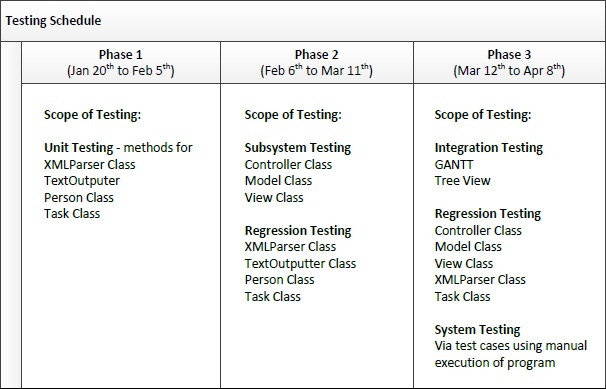
\includegraphics[scale=1]{Schedule.jpg} \end{center}
\label{fig:testing-schedule}
\caption{Testing Schedule}

\end{figure}

\subsubsection{Resources Used}

\begin{figure}[htbp]

\begin{center} 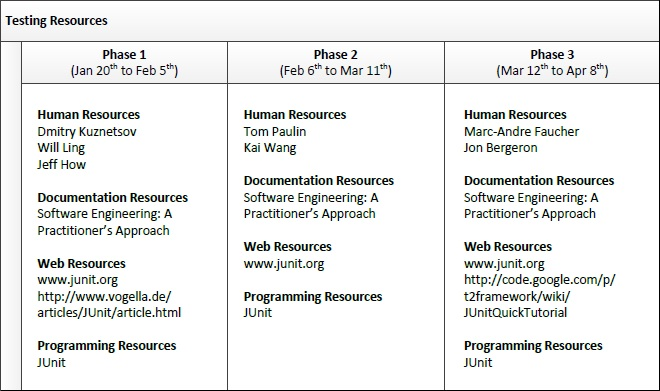
\includegraphics[scale=1]{Resources.jpg} \end{center}
\label{fig:testing-resources}
\caption{Testing Resources}

\end{figure}

\section{Test Results}
\subsubsection{Objective} 
{
Test system requirements to verify that they are operational and met by the implementation.
}
\subsubsection{Requirements Tested} 
{
  {\bf F1} Only one person should be logged in at a time.
    After increment 1, this requirement was deemed unnecessary.

  {\bf F2} A view of tasks in the company is to be shown to the user in order for him to manage
them.
    The table view is operational. Tested via manual executions of the user interface.  

  {\bf F3} The user is to be able to enter a new task.

Tested via manual executions of the user interface. Empty task added in Task view.

  {\bf F4} The user is to be able to remove a previously created task.
    Tested via manual executions of the user interface.

Initial testing resulted in three failures:

1. Removal of task did not update People View appropriately. Project was not removed from employee data.

  {\bf F5} The user is to be able to modify a previously created task.

Tested via manual executions of the user interface.

Initial testing resulted in three failures:

1. Verifying the correct format of data inputted into the system.

2. Inconsistency in dates between the Task View and XML document.

3. Inconsistency in data between the Task View and Person View. Changing project duration in Task View did not update employee's hours in Person View.

   {\bf F6} The user is to be able to view a Tree graph of tasks.
    The tree view is operational. Tested via manual executions of the user interface.  

   {\bf F7} The user is to be able to view a Gantt chart of tasks.
    The gantt view is operational. Tested via manual executions of the user interface.  

   {\bf F8} The user must be able to manage employees on a task.

Tested via manual executions of the user interface.

Initial testing resulted in a failure:

1. Management of employees did not update People View appropriately.

   {\bf F9} The user must be able to assign employees to a task.

Tested via manual executions of the user interface.

Initial testing resulted in a failure:

1. Assignment of employees did not update People View appropriately.


  {\bf F10} The user must be able to view a list of employees in the company with their respective data.
    The Person View is operational. Tested via manual executions of the user interface.  

  {\bf F11} The user is to be able to add a new employee.
    After increment 1, this requirement was deemed unnecessary.

  {\bf F12} The user is to be able to remove an employee.
    After increment 1, this requirement was deemed unnecessary.

  {\bf F13} The user must be able to withdraw employees from a task.
    Tested via manual executions of the user interface.

Initial testing resulted in a failure:

1. Withdrawal of employees did not update People View appropriately in regards to allocating hours.
}
\subsubsection{Conclusion}
{
In regards to requirements deemed necessary, any failures were communicated with the programmers, who fixed the code. Follow-up tests were performed to ensure the issues were resolved. The testers are satisfied with the final results.
}

\section{References}

\appendix

\section{Description of Input Files}
\subsection{People.xml}
{
$<$people$>$ : Root node used to specify the beginning of the listing of people

$<$person$>$ : Node used to specify a new person

$<$identifier$>$ : A unique, alphanumberic identifier for each person

$<$fname$>$ : Node used to store the first name of the person

$<$lname$>$ : Node used to store the last name of the person

$<$jobtitle$>$ : Node used to track the job title of the person. Used to differentiate betweenroles

$<$jobdescription$>$ : Node used for the person's job description.

$<$clearance$>$ : Node used to specify the clearance a person within the organization. Restricts permission based on value. 0 - Employee, 1 - Manager, 2 - Administrator
}
\subsection{Tasks.xml}
{
$<$tasks$>$ : Root node used to specify the beginning of the listing of tasks

$<$task$>$ : Node used to specify a new task

$<$identifier$>$ : A unique, alphanumberic identifier for each task

$<$title$>$ : Node to store a short title for the task

$<$description$>$ : Node to store a full description for the task

$<$startdate$>$ : Node to store the appropriate start date for the task

$<$duration$>$ : The duration, in hours of the task.

$<$deliverable$>$ : The expected physical deliverable upon task completion

$<$deadline$>$ : The date by which the task must be completed

$<$parentDependencyId$>$ : The identifier of the task which must be completed before this task can be completed.

$<$parent$>$ : The identifier for which this task is a subtask.

$<$peopleassigned$>$ : A listing of the individuals assigned to the task. The duration will be split evenly among assignees.

$<$id$>$ : The corresponding identifier for each person assigned

$<$completion$>$ : The percentage of completion for the task
}
\subsection{Sample Invalid XML Files}
{

 $<$ ?xml version=``1.0"? $>$ 
\\ $<$ !-- COMP 354 Project - Group 1 - XML People File-- $>$ 
\\ $<$ people $>$ 
\\ \tab$<$ person $>$ 
\\ \tab\tab $<$ identifier $>$ .0 $<$ /identifier $>$ 
\\ \tab\tab $<$ fname $>$ K.ai $<$ /fname $>$ 
\\ \tab\tab $<$ lname $>$ W56ang $<$ /lname $>$ 
\\ \tab\tab $<$ jobtitle $>$  Tes\%\$t Title $<$ /jobtitle $>$ 
\\ \tab\tab $<$ jobdescription $>$ Test .Job Description $<$ /jobdescription $>$ 
\\ \tab\tab $<$ clearance $>$ gh0 $<$ /clearance $>$ 
\\ \tab$<$ /person $>$ 
\\ \tab$<$ person $>$ 
\\ \tab\tab $<$ identifier $>$ h1 $<$ /identifier $>$ 
\\ \tab\tab $<$ fname $>$ Dmitry $<$ /fname $>$ 
\\ \tab\tab $<$ lname $>$ Kuznetsov $<$ /lname $>$ 
\\ \tab\tab $<$ jobtitle $>$ Test \^{} \%\$ Title $<$ /jobtitle $>$ 
\\ \tab\tab $<$ jobdescription $>$ Test Job.. Description $<$ /jobdescription $>$ 
\\ \tab\tab $<$ clearance $>$ dgfh0 $<$ /clearance $>$ 
\\ \tab$<$ /person $>$ 
\\ \tab$<$ person $>$ 
\\ \tab\tab $<$ identifier $>$ h2 $<$ /identifier $>$ 
\\ \tab\tab $<$ fname $>$ Wi5lliam $<$ /fname $>$ 
\\ \tab\tab $<$ lname $>$ Lin5g $<$ /lname $>$ 
\\ \tab\tab $<$ jobtitle $>$ Test \%\$\^Title $<$ /jobtitle $>$ 
\\ \tab\tab $<$ jobdescription $>$ Test Job\%\$\^{} Description $<$ /jobdescription $>$ 
\\ \tab\tab $<$ clearance $>$ 0hfd $<$ /clearance $>$ 
\\ \tab$<$ /person $>$ 
\\ \tab$<$ person $>$ 
\\ \tab\tab $<$ identifier $>$ h3 $<$ /identifier $>$ 
\\ \tab\tab $<$ fname $>$ Jef46frey $<$ /fname $>$ 
\\ \tab\tab $<$ lname $>$ Ho56w $<$ /lname $>$ 
\\ \tab\tab $<$ jobtitle $>$ Test \%\^{}Title $<$ /jobtitle $>$ 
\\ \tab\tab $<$ jobdescription $>$ Test J\^{}\%\$ob Description $<$ /jobdescription $>$ 
\\ \tab\tab $<$ clearance $>$ .. $<$ /clearance $>$ 
\\ \tab$<$ /person $>$ 
\\ \tab$<$ person $>$ 
\\ \tab\tab $<$ identifier $>$ 4\% $<$ /identifier $>$ 
\\ \tab\tab $<$ fname $>$ Jona56than $<$ /fname $>$ 
\\ \tab\tab $<$ lname $>$ Berg566eron $<$ /lname $>$ 
\\ \tab\tab $<$ jobtitle $>$ Test \%\$\^{}Title $<$ /jobtitle $>$ 
\\ \tab\tab $<$ jobdescription $>$ Test\%\$\^{}  Job Description $<$ /jobdescription $>$ 
\\ \tab\tab $<$ clearance $>$ hf0 $<$ /clearance $>$ 
\\ \tab$<$ /person $>$ 
\\ \tab$<$ person $>$ 
\\ \tab\tab $<$ identifier $>$ dfh5 $<$ /identifier $>$ 
\\ \tab\tab $<$ fname $>$ Al354ain $<$ /fname $>$ 
\\ \tab\tab $<$ lname $>$ Sa54kha $<$ /lname $>$ 
\\ \tab\tab $<$ jobtitle $>$ Test \$\%Title $<$ /jobtitle $>$ 
\\ \tab\tab $<$ jobdescription $>$ Test J..ob Description $<$ /jobdescription $>$ 
\\ \tab\tab $<$ clearance $>$ gdg0 $<$ /clearance $>$ 
\\ \tab$<$ /person $>$ 
\\ \tab$<$ person $>$ 
\\ \tab\tab $<$ identifier $>$ g6 $<$ /identifier $>$ 
\\ \tab\tab $<$ fname $>$ Marc-An543dre $<$ /fname $>$ 
\\ \tab\tab $<$ lname $>$ Fauch45er $<$ /lname $>$ 
\\ \tab\tab $<$ jobtitle $>$ Test T\$\%itle $<$ /jobtitle $>$ 
\\ \tab\tab $<$ jobdescription $>$ Test Job\#\$\% Description $<$ /jobdescription $>$ 
\\ \tab\tab $<$ clearance $>$ g0 $<$ /clearance $>$ 
\\ \tab$<$ /person $>$ 
\\ \tab$<$ person $>$ 
\\ \tab\tab $<$ identifier $>$ g7 $<$ /identifier $>$ 
\\ \tab\tab $<$ fname $>$ T45homas $<$ /fname $>$ 
\\ \tab\tab $<$ lname $>$ Pa54ulin $<$ /lname $>$ 
\\ \tab\tab $<$ jobtitle $>$ Te\$\#\%\$st Title $<$ /jobtitle $>$ 
\\ \tab\tab $<$ jobdescription $>$ Test\#\$\% Job Description $<$ /jobdescription $>$ 
\\ \tab\tab $<$ clearance $>$ fg0 $<$ /clearance $>$ 
\\ \tab$<$ /person $>$ 
\\ $<$ /people $>$ 
\\ $<$ ?xml version=``1.0"? $>$ 
\\ $<$ !DOCTYPE tasks SYSTEM ``tests\textbackslash resources\textbackslash TASK\_DTD\_SCHEMA.dtd" $>$ 
\\ $<$ !-- COMP 354 Project - Group 1 - XML Task File-- $>$ 
\\ $<$ tasks $>$ 
\\ \tab$<$ t2ask $>$ 
\\ \tab    \tab $<$ identifier $>$ . $<$ /identifier $>$ 
\\ \tab    \tab $<$ title $>$ Modelling\% $<$ /title $>$ 
\\ \tab    \tab $<$ description $>$ \-\%Modelling for the game. Includes Character and Environment Modelling $<$ /description $>$ 
\\ \tab    \tab $<$ duration $>$ 175? $<$ /duration $>$ 
\\ \tab    \tab $<$ deliverable $>$ Zipped Folder. Containing\%\^{} all Models and Documentation $<$ /deliverable $>$ 
\\ \tab    \tab $<$ deadline $>$ .Feb 18, 2012 $<$ /deadline $>$ 
\\ \tab    \tab $<$ personassigned $>$ Kai, \$\%Tom $<$ /personassigned $>$ 
\\ \tab    \tab $<$ completion $>$ 0h $<$ /completion $>$ 
\\ \tab    \tab $<$ subtask $>$  $<$ /subtask $>$ 
\\ \tab$<$ /task $>$ 
\\ 
\\ \tab$<$ task $>$ 
\\ \tab    \tab $<$ identifier $>$ 1h $<$ /identifier $>$ 
\\ \tab    \tab $<$ title $>$ User .Interface $<$ /title $>$ 
\\ \tab    \tab $<$ description $>$ Design \^{}and creation of the user interface for the game. Includes the in-game HUD and front-end menus. $<$ /description $>$ 
\\ \tab    \tab $<$ duration $>$ .114 $<$ /duration $>$ 
\\ \tab    \tab $<$ deliverable $>$ Zipped Folder ContaininDF\#\$g all Interface files and Documentation $<$ /deliverable $>$ 
\\ \tab    \tab $<$ deadline $>$ jFeb 15, 2012 $<$ /deadline $>$ 
\\ \tab    \tab $<$ personassigned $>$ .Jonathon,\# Jeff $<$ /personassigned $>$ 
\\ \tab    \tab $<$ completion $>$ 0. $<$ /completion $>$ 
\\ \tab    \tab $<$ subtask $>$  $<$ /subtask $>$ 
\\ \tab$<$ /task $>$ 
\\
\\ \tab$<$ task $>$ 
\\ \tab    \tab $<$ identifier $>$ .2 $<$ /identifier $>$ 
\\ \tab    \tab $<$ title $>$ Tes\%ting $<$ /title $>$ 
\\ \tab    \tab $<$ description $>$ Testing for the\^\$ game. Included QA and Compliance testing $<$ /description $>$ 
\\ \tab    \tab $<$ duration $>$ 3645h6 $<$ /duration $>$ 
\\ \tab    \tab $<$ deliverable $>$ Completed\#\@\$ Testing checklist with bug reports. $<$ /deliverable $>$ 
\\ \tab    \tab $<$ deadline $>$ Feb 1.0, 2012 $<$ /deadline $>$ 
\\ \tab    \tab $<$ personassigned $>$ Willie, Dmitr\%\$y, Alain $<$ /personassigned $>$ 
\\ \tab    \tab $<$ completion $>$ 0. $<$ /completion $>$ 
\\ \tab    \tab $<$ subtask $>$  $<$ /subtask $>$ 
\\ \tab$<$ /task $>$ 
\\ 
\\ \tab$<$ task $>$ 
\\ \tab    \tab $<$ identifier $>$ 3. $<$ /identifier $>$ 
\\ \tab    \tab $<$ title $>$ Develop\$\%ment $<$ /title $>$ 
\\ \tab    \tab $<$ description $>$ Development of source code for th\$\%e game. Includes elements of gameplay, level design, etc. $<$ /description $>$ 
\\ \tab    \tab $<$ duration $>$ 20.0 $<$ /duration $>$ 
\\ \tab    \tab $<$ deliverable $>$ Zipped folder 56\%\^containing all main game files $<$ /deliverable $>$ 
\\ \tab    \tab $<$ deadline $>$ F eb 9, 2012 $<$ /deadline $>$ 
\\ \tab    \tab $<$ personassigned $>$ \%\^{}Tom, Jeff, Willie, Dmitry $<$ /personassigned $>$ 
\\ \tab    \tab $<$ completion $>$ .0 $<$ /completion $>$ 
\\ \tab    \tab $<$ subtask $>$  $<$ /subtask $>$ 
\\ \tab$<$ /task $>$ 
\\ 
\\ \tab$<$ task $>$ 
\\ \tab    \tab $<$ identifier $>$ .4 $<$ /identifier $>$ 
\\ \tab    \tab $<$ title $>$ Artificial \%Intelligence $<$ /title $>$ 
\\ \tab    \tab $<$ description $>$ Artificial InS@telligence $<$ /description $>$ 
\\ \tab    \tab $<$ duration $>$ 95gh0 $<$ /duration $>$ 
\\ \tab    \tab $<$ deliverable $>$ Zipped folde\#\$r containing algorithms and AI code $<$ /deliverable $>$ 
\\ \tab    \tab $<$ deadline $>$ F.eb 15, 2012 $<$ /deadline $>$ 
\\ \tab    \tab $<$ personassigned $>$ Kai, Jonatho\%n, Alain $<$ /personassigned $>$ 
\\ \tab    \tab $<$ completion $>$ 0\$\% $<$ /completion $>$ 
\\ \tab    \tab $<$ subtask $>$  $<$ /subtask $>$ 
\\ \tab$<$ /task $>$ 
\\ 
\\ \tab$<$ task $>$ 
\\ \tab    \tab $<$ identifier $>$ 5\^{} $<$ /identifier $>$ 
\\ \tab    \tab $<$ title $>$ Docum\$\#\%entation $<$ /title $>$ 
\\ \tab    \tab $<$ description $>$ All internal and \$\#external documentation for the game $<$ /description $>$ 
\\ \tab    \tab $<$ duration $>$ 145\$\#\%00 $<$ /duration $>$ 
\\ \tab    \tab $<$ deliverable $>$ Zipped folder .containing al\#l documentation, including user manuals $<$ /deliverable $>$ 
\\ \tab    \tab $<$ deadline $>$ F.eb 21, 2012 $<$ /deadline $>$ 
\\ \tab    \tab $<$ personassigned $>$ Alain,\# Dmitry $<$ /personassigned $>$ 
\\ \tab    \tab $<$ completion $>$ .0 $<$ /completion $>$ 
\\ \tab    \tab $<$ subtask $>$  $<$ /subtask $>$ 
\\ \tab$<$ /task $>$ 
\\ 
\\ \tab$<$ task $>$ 
\\ \tab    \tab $<$ identifier $>$ 6h $<$ /identifier $>$ 
\\ \tab    \tab $<$ title $>$ Integra.\$\%tion $<$ /title $>$ 
\\ \tab    \tab $<$ description $>$ Integratio\#\$@\#n of all features from all tasks $<$ /description $>$ 
\\ \tab    \tab $<$ duration $>$ 2345\$\%50 $<$ /duration $>$ 
\\ \tab    \tab $<$ deliverable $>$ \$\%Finalized game executable $<$ /deliverable $>$ 
\\ \tab    \tab $<$ deadline $>$ 4Feb 30, 2012 $<$ /deadline $>$ 
\\ \tab    \tab $<$ personassigned $>$ Tom.\#, Jeff, Willie, Jonathon, Kai, Alain $<$ /personassigned $>$ 
\\ \tab    \tab $<$ completion $>$ .0 $<$ /completion $>$ 
\\ \tab    \tab $<$ subtask $>$  $<$ /subtask $>$ 
\\ \tab$<$ /task $>$ 
\\ $<$ /tasks $>$ 
}

\section{Description of Output Files}
\subsection{People.txt}
\begin{lstlisting}

The list of people with a summary of their names, the total amount
of time spent on all projects, and the specific projects to which
they are assigned. Sample format:

Name                    | Total Hours | Project List
--------------------------------------------------------------
LName , FName           |         X.X | A, B, C

\end{lstlisting}
\section{List of Requirements}

\subsection{Functional Requirements}
\subsubsection{F1}
{
 Only one person should be logged in at a time.
}
\subsubsection{F2}
{
A view of tasks in the company is to be shown to the user in order for him to manage them.
}
\subsubsection{F3}
{
The user is to be able to enter a new task.
}
\subsubsection{F4}
{
The user is to be able to remove a previously created task.
}
\subsubsection{F5}
{
The user is to be able to modify a previously created task.
}
\subsubsection{F6}
{
The user is to be able to view a dependency graph of tasks.
}
\subsubsection{F7}
{
The user is to be able to view a Gantt chart of tasks.
}
\subsubsection{F8}
{
The user must be able to manage employees on a task.
}
\subsubsection{F9}
{
The user must be able to assign employees to a task.
}
\subsubsection{F10}
{
The user must be able to view a list of employees in the company in order for him to manage them.
}
\subsubsection{F11}
{
The user is to be able to add a new employee.
}
\subsubsection{F12}
{
The user is to be able to remove an employee.
}
\subsubsection{F13}                                                                         
{
The user must be able to withdraw employees from a task.
}
\subsection{C.2 - Non-Functional Requirements}
\subsubsection{N1}
{
The system must know who the user is in order to order the appropriate options.
}
\subsubsection{O1}
{
It shall be possible to run the system on any computer system that runs the JVM.
}
\end{document}
